\chapter{Implementation}
The virtual globe rendering system was implemented as a separate module, programmed in C++ for OpenSpace which, if desired, can be opted out when building the software. The implementation defines a namespace with all the necessary data structures, classes and functionality specifically related to globe rendering. The basic structure of a \class{Renderable Globe} with its necessary components is illustrated as a UML diagram in figure \ref{fig:renderableglobe}.

\begin{figure}[htbp]
    \centering
    \begin{subfigure}[bt]{0.8\textwidth}
        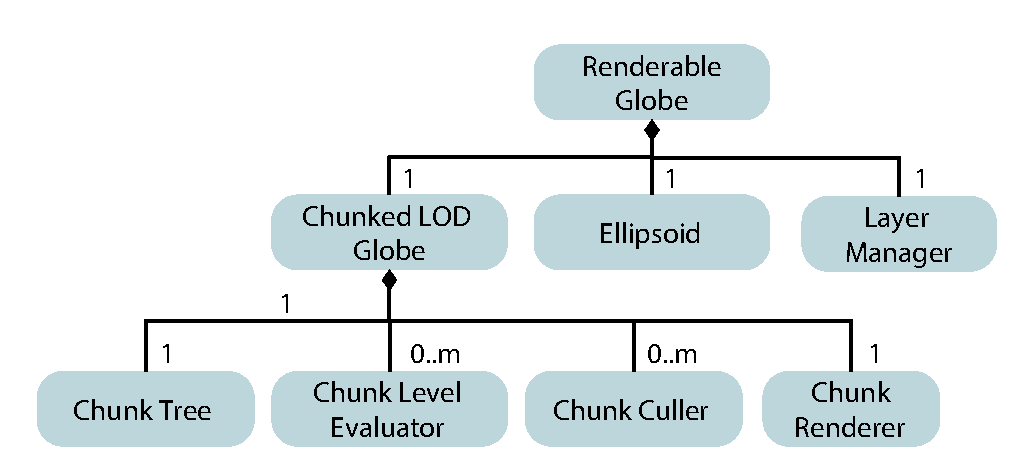
\includegraphics[width=\textwidth]{figures/implementation/renderable_globe.pdf}
    \end{subfigure}
    \caption{Overviewing class diagram of \class{Renderable Globe} and its related classes.}
    \label{fig:renderableglobe}
\end{figure}

The base of the globe renderer uses a modified version of Cozzi and Rings Chunked LOD algorithm. The globe is tessellated as an ellipsoid with a geometrical grid using geodetic map projection.

The full LOD rendering system required several components of different complexity to be implemented. All components will be described in detail in this chapter.

\section{Reference Ellipsoid}
The \class{Ellipsoid} class was implemented to handle all geographic related calculations.  These calculations include conversions between geodetic and cartesian coordinates and different kinds of projections onto the ellipsoid surface. These calculations are sped up by internal caching of a range of precalculated values. Cozzi and Ring provide a complete reference on the implementation \cite[p. 17]{cozzi11}.

The \class{Ellipsoid} uses several geographically related classes, which were used in multiple places within the implementation. These are:
\begin{enumerate}
	\item \class{Angle} - Handles angle related arithmetics, normalizations and unit abstractions (degrees and radians)
	\item \class{Geodetic2} - Represents a 2D geodetic coordinate (latitude, longitude)
	\item \class{Geodetic3} - Represents a 3D geodetic coordinate (latitude, longitude, altitude)
	\item \class{GeodeticPatch} - Represents a rectangular region in geodetic space
\end{enumerate}

\section{Chunked LOD}
The base of the chunked LOD algorithm revolves around the self updating chunk tree. The chunk tree is a data structure built up of \class{Chunk Node}s which have the ability to split or merge dynamically. Besides storing four \class{Chunk Node} children, each \class{Chunk Node} stores a \class{Chunk}.

\subsection{Chunks}
As opposed to the definition of chunks in the background section \ref{section:chunkedlodbacground}, this implementation of chunks is very lightweight - it does not store any texture or triangle mesh data. Instead, it stores the information needed to query texture tiles from local in-memory caches. In the implementation suggested by Cozzi and Ring, terrain triangle meshes are stored in each chunk. In the case of this implementation however, all terrain is rendered using height mapped vertex grids. Thus there is no need for each chunk to store their own vertex arrays. Instead they can simply share one single instance of a vertex grid within a whole chunk tree. This means that vertices need to be offset by height mapping on the GPU which makes it possibly to dynamically change height datasets that does not require pre processing before they can be used for rendering.

The most important part of the chunked LOD algorithm is the ability to dynamically select which chunks to split or merge. 

\subsection{Chunk Selection}
\label{section:chunkselection}
The chunk tree is automatically reshaped depending on the virtual camera. A chunk node splits, merges or remain the same depending on the chunk's error metric for the current LOD. Three different approaches for calculating the error metric were implemented. By letting the user dynamically adjust a LOD scale factor, performance can be weighted against detail level.

\subsubsection{By Distance}
Letting the error depend on the distance between the closest point on the chunk, and the camera $d$ as in Equation \ref{eq:loddistance}, will lead to more or less constant size of the chunks in screen space.

\begin{equation}
	\label{eq:loddistance}
	e = l - log_2(\frac{s}{d}),
\end{equation}
where $e$ is the error, $l$ is the current level of the chunk, $s$ is a LOD scaling factor and $d$ is the distance between the closest point of the chunk and the camera. The closest point of the chunk can be either a corner or a point along one of the chunk edges. Using this distance as an error metric leads to bigger chunks farther from the camera where less detail is needed.


\subsubsection{By Projected Area}
Another error metric is the area that the chunk takes up on the screen. The bigger the area, the bigger the error. 

The error must not be dependent of the direction of the camera. This is because a chunk rendered on a multi screen display, such as a dome, should not have different errors between two or more screens which might lead to different levels and tearing between screens. Therefore the chunk is projected on a unit sphere and not a view plane which would lead to view direction dependent error metrics.

\begin{figure}[htbp]
    \centering
    \begin{subfigure}[bt]{0.5\textwidth}
        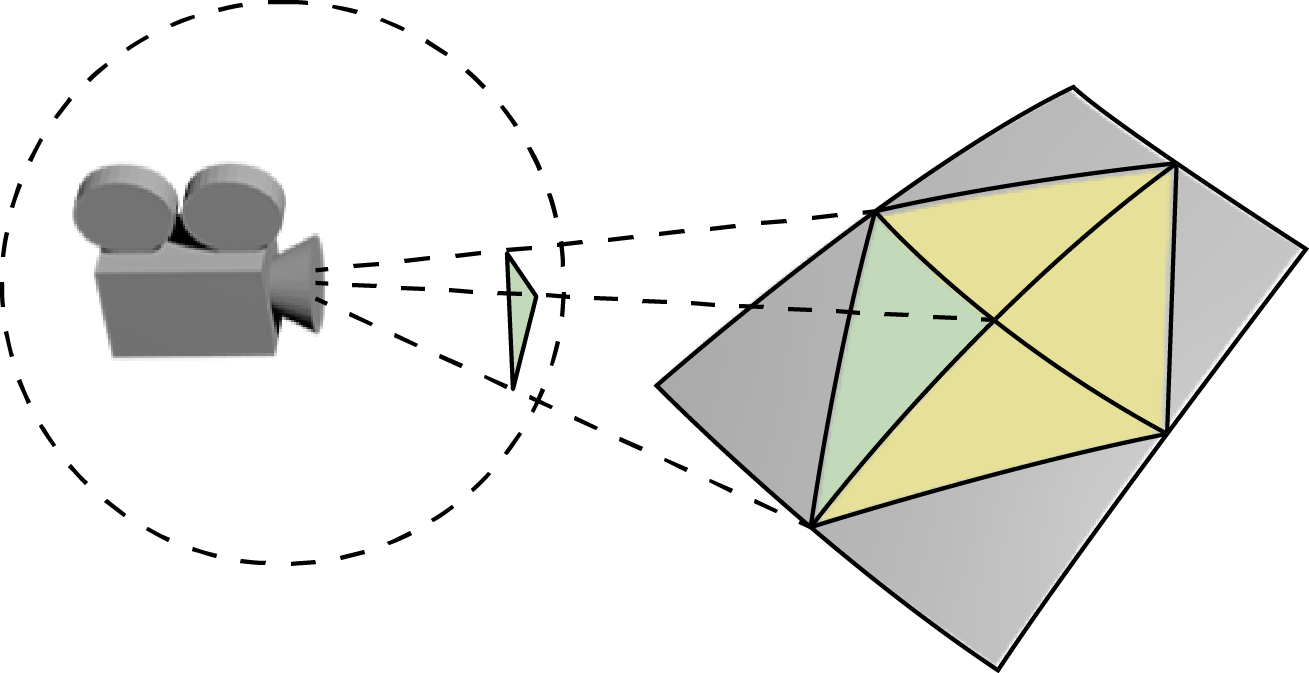
\includegraphics[width=\textwidth]{figures/implementation/chunklod/projectedarea.png}
    \end{subfigure}
    \caption{Triangle with the area 1/8 of the chunk projected onto a unit sphere. The area is used to approximate the solid angle of the chunk used as an error metric when selecting chunks to render}
    \label{fig:chunkprojarea}
\end{figure}

The projected area is a solid angle approximated by extracting three points on the chunk and projecting them on a unit sphere centered in the camera position. The three points define the closest of the four center triangles on the chunk, see figure \ref{fig:chunkprojarea}. It is important that the triangle chosen for approximating the projected area can never have two vertices on the same upper or lower most edge. Such triangles (colored gray in figure \ref{fig:chunkprojarea}) may collapse down to a line and hence have zero area for chunks at the poles, thus cannot be used to approximate the area of the full chunk.

The actual approximated solid angle is the projected triangle area multiplied by eight to accommodate a full chunk. This area is then subtracted by a constant value and scaled by a LOD scale factor to give similar LOD scaling as the distance dependent chunk selection.

\subsection{Chunk Tree Growth Limitation}
The chunk selection algorithms described above determine a suitable level of detail based on the camera. This causes chunks that have too large of an error to split. However, splitting a chunk will not result in higher level of detail unless the corresponding higher tile data is also currently available for rendering. Therefore, the growth of the chunk tree is be limited by checking if there is any tile data there in the first place. This is useful in two scenarios:

\begin{enumerate}
\item Rendering of sparse map datasets which contain geographical regions where there are no data
\item Rendering of map datasets which are queried from remote servers; there will always be some delay where the queried map data is not yet available
\end{enumerate}

Being able to limit the chunk tree in these two scenarios, unnecessary chunk rendering calls is be avoided.

\subsection{Chunk Culling}
Given a chunk tree with chunks selected based on the camera position, each chunk can be tested using chunk cullers to determine if they are ``cullable'' and therefore can be set to invisible so that the chunk renderer will not bother in rendering them. The two implemented chunk cullers are the frustum culler and the horizon culler. They both rely on, and have access to, minimum and maximum values of the chunk's height maps. 

\subsubsection{Frustum Culling}
Frustum culling is implemented by first calculating a convex bounding polyhedron for the chunk to be tested. The bounding volume is calculated on the fly and takes into account any enabled height maps used to displace the vertices, making sure it fully encapsulates the displaced chunk vertices. The polyhedron is built up of eight vertices which are transformed to normalized device coordinates (NDC) using the view-projection matrix of the camera followed by perspective division. Once in NDC, an axis aligned bounding box (AABB) for the vertices is extracted. This AABB can then be tested against the screen bounds to determine if the chunk is outside the camera's field of view, and thus is cullable. This is illustrated in figure \ref{fig:frustumculling}.

\begin{figure}[htbp]
    \centering
    \begin{subfigure}[bt]{1.0\textwidth}
        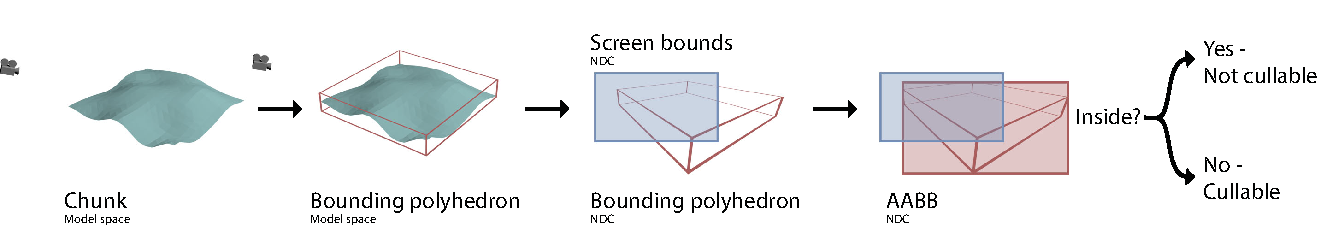
\includegraphics[width=\textwidth]{figures/implementation/chunklod/frustumculling.pdf}
    \end{subfigure}
    \caption{Frustum culling algorithm. This chunk cannot be frustum culled.}
    \label{fig:frustumculling}
\end{figure}

\subsubsection{Horizon Culling}
Given an object in position $\vec{p}$ with a bounding radius $r$ on the surface of the globe, it can be determined if it is completely behind the globe's horizon or not. The calculations are simplified by approximating the globe as a sphere using the minimum radius $r_g$ of its ellipsoid. Using the minimum radius and not a bigger number ensures that false occluding (chunks marked as invisible actually being visible) is not possible \cite[p. 393]{cozzi11}. The minimum allowed distance $l$ to the object can be calculated as the distance to the horizon $l_h$ added to the minimum allowed distance to the object from the horizon $l_m$. See figure \ref{fig:horizonculling}. Once the minimum allowed distance is calculated it can be compared to the actual distance to the object to determine if it is cullable or not.

\begin{figure}[htbp]
    \centering
    \begin{picture}(130,130)
        \put(0,0){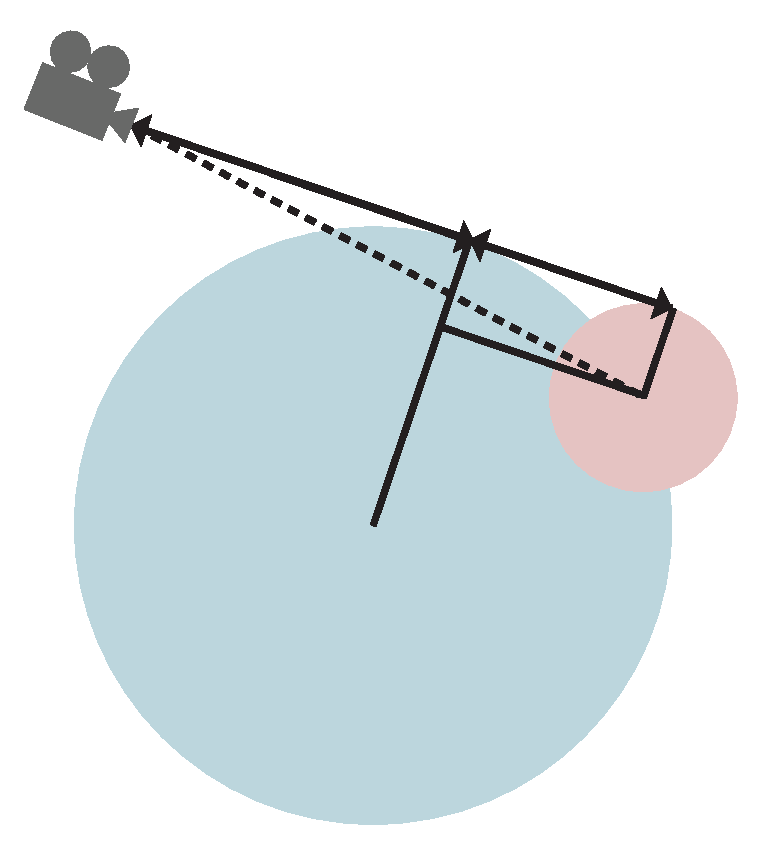
\includegraphics[width=0.4\textwidth]{figures/implementation/chunklod/horizonculling.pdf}}
        \put(60,145){$l_h$}
        \put(115,125){$l_m$}
        \put(135,95){$r$}
        \put(70,95){$r_g$}
        \put(130,80){$\vec{p}$}
        
    \end{picture}
    \caption{Horizon culling is performed by comparing the length $l_h+l_m$ with the actual distance between the camera position and the object at position $\vec{p}$.}
    \label{fig:horizonculling}
\end{figure}

When culling chunks, the closest position on the chunk is used as the position $\vec{p}$ and the bounding height value as $r$.

\section{Reading and Tiling Image Data}
Fetching the right texture and preparing it for rendering onto chunks is a fairly complicated process. Before digging into the details of this process, there are three concepts that need to be established, as they will be referred to throughout the description of the texture pipeline. These are:

\begin{enumerate}
	\item \textbf{\class{Tile Index}} - A tuple of three integers $(level, x, y)$ indexing a specific map region on the globe
	\item \textbf{\class{Raw Tile}} - A texture carved out to fit the geographical region of a specific chunk, along with meta data. Each \class{Raw Tile} is associated with a \class{Tile Index}. They can be instantiated concurrently
	\item \textbf{\class{Tile}} - Like a \class{Raw Tile}, but the texture data is uploaded to the GPU and ready to use for rendering (unless it has a status not equal to ``OK''). As opposed to \class{Raw Tiles}, tiles rely on an OpenGL context and must therefore be initialized on the rendering thread
\end{enumerate}

All chunk height and texture data are represented using \class{Tiles}. \class{Tiles} are created on the client side (i.e. in OpenSpace) on the fly when they are needed. As the pixel data may need to be read from disk or even requested from remote servers, the whole tile preparation pipeline was implemented to be executed on separate threads in order to avoid blocking of the rendering thread with image data reads. 

During the iterative process of developing the texture tile pipeline, three layers of abstraction were introduced in order to deal with the fairly high complexity. See table \ref{table:tilepipeline}.

\begin{center}
  \begin{table}
  \caption[]{Abstraction layers used in the texture data pipeline}
    \label{table:tilepipeline}
  \resizebox{\textwidth}{!}{\begin{tabular}{| c | c | c | c |}
    \hline
     Layer & \textbf{Component} 	& \textbf{Responsibility} & \textbf{Input --> Output} \\ \hline 
    3 & \class{Async Tile Dataset} 	& Async \class{Raw Tile} fetching  & \class{TileIndex} --> \class{Raw Tile} \\ \hline
    2 & \class{Tile Dataset}        & Tiling, georeferencing,  & \class{TileIndex} --> \class{Raw Tile} \\ 
     &         & preprocessing &  \\ \hline
    1 & GDAL         		& Image formats, I/O Operations, & pixel region --> pixel data \\
     &          		& georeferencing &  \\
    \hline
  \end{tabular}}
  \end{table}
\end{center}

The subsequent sections of this chapter will cover each abstraction layer in more detail, starting from the bottom and going up the stack.

\subsection{GDAL}
Geospatial Data Abstraction Library (GDAL) is an open source library providing a uniform interface for reading, manipulating and writing geospatial data in the form of raster and vector data models \cite{gdal}. GDAL is used as an abstraction layer between all the map formats and the representation of tile datasets. It provides an interface allowing client code to specify pixel regions within a dataset to read from, independent of the underlying image format. GDAL can also be used for disk based caching of data from remote servers. Reading pixel data using the GDAL RasterIO interface requires a set of parameters listed below and illustrated in figure \ref{fig:gdalio}:

\begin{enumerate}
	\item A map overview to read pixel data from (if the dataset has overviews)
	\item A pixel region within that map overview to read pixels from
	\item The raster band(s) (e.g., color channels) to read
	\item A pointer to sufficient user allocated memory where GDAL can write the output of the read operation
	\item The pixel region to write the output pixel data. The size of the pixel data to be written may differ from the pixel region to read from, in which case GDAL will resample and interpolate the pixel data automatically
	\item The layout (i.e., pixel spacing, raster band spacing and line spacing)
	\item The data type to retrieve the pixel data in
\end{enumerate}

\begin{figure}[htbp]
    \centering
    \begin{subfigure}[bt]{1.0\textwidth}
        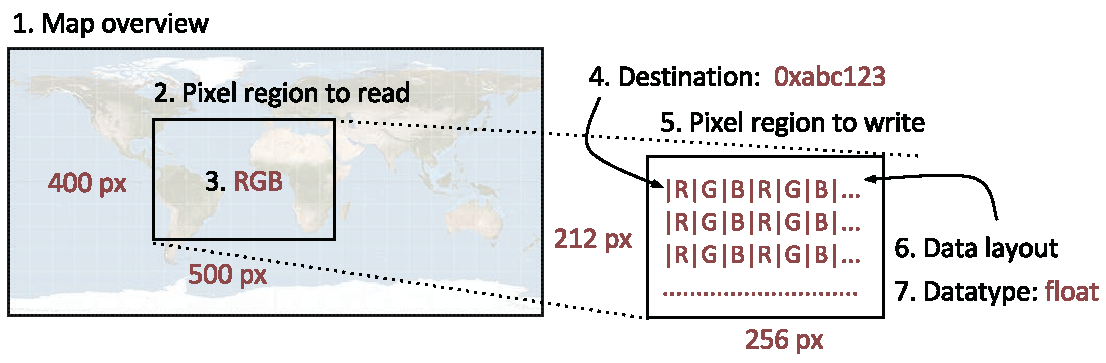
\includegraphics[width=\textwidth]{figures/implementation/pipeline/gdalio.pdf}
    \end{subfigure}
    \caption{The required GDAL RasterIO parameters. Figure adapted from \cite{mapprojections}}
    \label{fig:gdalio}
\end{figure}

With the given input parameters shown in figure \ref{fig:gdalio}, the resulting output would be the pixel data of the requested image region written with the pixel layout parameters to the provided memory block. The output is illustrated in figure \ref{fig:gdalioresult}.

\begin{figure}[htbp]
    \centering
    \begin{subfigure}[bt]{0.5\textwidth}
        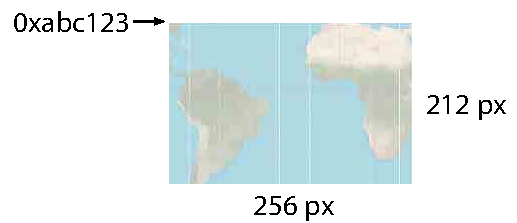
\includegraphics[width=\textwidth]{figures/implementation/pipeline/gdalioresult.pdf}
    \end{subfigure}
    \caption{Result of GDAL raster IO. Figure adapted from \cite{mapprojections}}
    \label{fig:gdalioresult}
\end{figure}

Using the RasterIO interface on an open GDAL dataset, the notion of image format is completely abstracted away. This is a great advantage which also allows GDAL to support sparse datasets. Appendix \ref{appendix:localpatches} goes through a detailed example of how to use GDAL for reading sparse datasets such as local, georeferenced, image patches of high resolution.

GDAL also provides the coefficients of a geo-transform which defines the mapping from raster coordinates to georeferenced coordinates. The geo-transform can be inverted to transform a georeferenced region to raster space when specifying the area of an image tile to read.

\subsection{Tile Dataset}
\class{Tile Dataset}s carves out \class{Raw Tile}s from GDAL datasets based on a \class{Tile Index}. Along with the pixel data, the served \class{Raw Tile}s also contain some metadata. The metadata includes an error code if the read operation failed and some basic information about to read pixel data, such as minimum and maximum pixel values. Figure \ref{fig:tiledataset} illustrates how the process from \class{Tile Index} to \class{Raw Tile} is carried out. There are three gray subroutines; \emph{Get IO description}, \emph{Read image data} and \emph{Calculate metadata}. These subroutines are explained below.

\begin{figure}[htbp]
    \centering
    \begin{subfigure}[bt]{0.8\textwidth}
        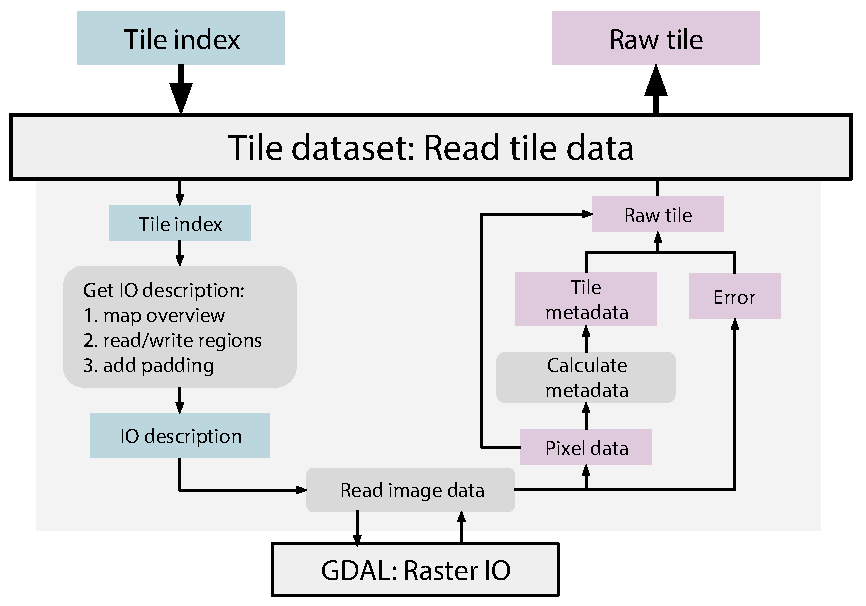
\includegraphics[width=\textwidth]{figures/implementation/pipeline/tiledataset.pdf}
    \end{subfigure}
    \caption{The tile dataset pipeline takes a tile index as input, interfaces with GDAL and returns a raw tile}
    \label{fig:tiledataset}
\end{figure}

\subsubsection{Get IO Description}
The IO description contains all tile specific information needed to perform a map read request using GDAL. This includes the pixel region to read, and where to store the result. The derivation of this information is summarized in the following steps, and illustrated in figure \ref{fig:getiodescription}.

\begin{figure}[htbp]
    \centering
    \begin{subfigure}[bt]{0.9\textwidth}
        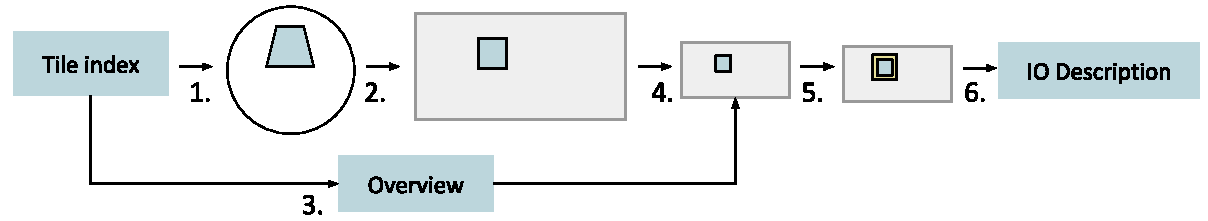
\includegraphics[width=\textwidth]{figures/implementation/pipeline/getiodescription.pdf}
    \end{subfigure}
    \caption{Overview of the calculation of an IO description. Figure adapted from \cite{mapprojections}}
    \label{fig:getiodescription}
\end{figure}

\begin{enumerate}
\item Calculate a \class{Geodetic Patch} from \class{Tile Index}
\item Calculate the pixel coordinates for the patch in raster coordinate space
\item Calculate a suitable map overview
\item Transform pixel region to map overview
\item Add padding to the down scaled pixel region
\item Finalize the gathered data to an IO description object.
\end{enumerate}

In the scheme in figure \ref{fig:getiodescription}, step 1 is performed using equation \ref{eq:latlongindex},

\begin{equation}
\label{eq:latlongindex}
\begin{split}
\phi_{NE} = 2\pi y / 2^{level} \\
\theta_{NE} = 2\pi x / 2^{level} \\
side = 2\pi / 2^{level},
\end{split} 
\end{equation}

where $\phi_{NE}$ and $\theta_{NE}$ are the latitude and the longitude of the north east corner of the tile and $side$ is the side length of the tile.

Calculating the corresponding GDAL overview is done according to equation \ref{eq:overview},

\begin{equation}
\label{eq:overview}
Overview(level) = N - level - 1 - log_2(size_{tile} / size_{map}),
\end{equation}

where $level$ is given by the provided \class{Tile Index}, $N$ is the total number of overviews in the dataset, $size_{tile}$ is a configurable constant defining the preferred pixel size of a tile and $size_{map}$ is the size of the full map in pixels. The sizes can be either along the $x-$ or $y-$ axis. In the implementation the $x-$axis is used.

Pixel coordinates can easily be transformed across map overviews using equation \ref{eq:overview}.

\begin{equation}
\label{eq:overview}
p_{n} = p_{m} \times 2^{m-n}
\end{equation}

Where $n$ is the destination map overview and $m$ is the source map overview. This is used for downscaling the pixel region in step 4, where $n$ is the calculated suitable overview and $m$ is zero (i.e. the full map). 

Padding is added to the pixel region in order to perform correct interpolation of pixel values across different tiles later during rendering. However, this may cause the pixel region to extend outside the map region. Therefore the last finalize step also handles wrapping of the pixel region before returning the final IO description. The wrapping used is a CPU implementation of $GL\_REPEAT$.

\subsubsection{Tile Meta Data}
As mentioned, \class{Tile Dataset}s can be configured to calculate some metadata on the fly based on the pixel data that has been read. The metadata includes minimum and maximum pixel values within the pixel data and whether or not the pixel data contains missing-data values. Having access to minimum and maximum values for height layer tiles is required for the culling to be performed correctly since the cullers rely on having bounding boxes for the chunks. The meta data can not be requested directly from GDAL since the tiling can differ from the underlying image tiling abstracted away by GDAL. Calculating the meta data had to be performed by explicitly looping through all the pixel values on the client side. 

\subsubsection{Summary}
To summarize, the implementation of \class{Tile Dataset} allow reading pixel data from a GDAL dataset corresponding to a specific \class{Tile Index}, along with metadata unless opted out. The \class{Raw Tile}s that are served are padded in order to perform smooth pixel blending between different tiles. \class{Raw Tile}s are not available for rendering since the data is not yet on the GPU.

\subsection{Async Tile Dataset}
\class{Async Tile Dataset}s utilize a shared thread pool and own a \class{Tile Dataset}. It provides a concurrent job posting interface for concurrent reads within the \class{Tile Dataset}. It has two important funcionalities: 1) enqueueing tile read jobs and 2) collect finished tile read jobs. Reading \class{Raw Tile}s on separate threads ensures that the render thread will not be delayed by image data requests, see figure \ref{fig:asynctiledataset}.

\begin{figure}[htbp]
    \centering
    \begin{subfigure}[bt]{0.6\textwidth}
        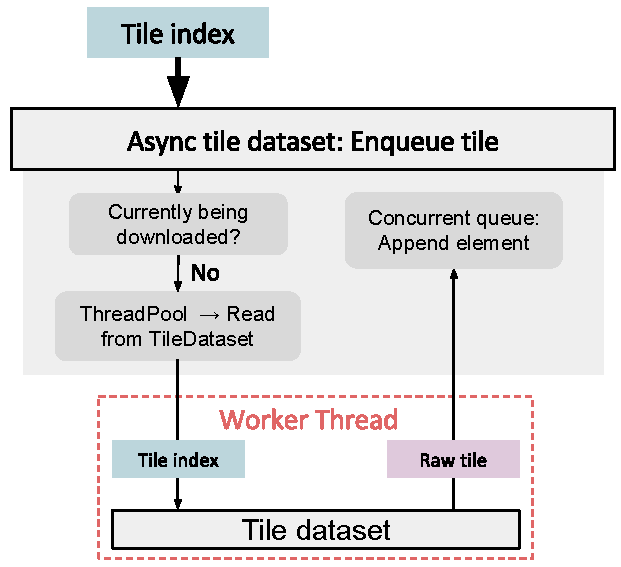
\includegraphics[width=\textwidth]{figures/implementation/pipeline/asynctiledataset.pdf}
    \end{subfigure}
    \caption{Asynchronious reading of Raw tiles can be performed on separate threads. When the tile reading job is finished the raw tile will be appended to a concurrent queue}
    \label{fig:asynctiledataset}
\end{figure}

\begin{figure}[htbp]
    \centering
    \begin{subfigure}[bt]{0.6\textwidth}
        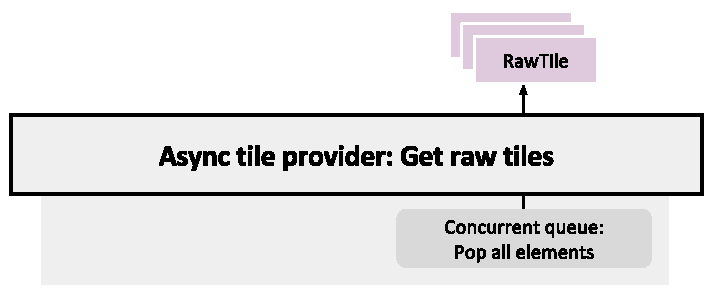
\includegraphics[width=\textwidth]{figures/implementation/pipeline/asynctiledataset_gettiles.pdf}
    \end{subfigure}
    \caption{Retrieving finished Raw tiles}
    \label{fig:asynctiledataset2}
\end{figure}

The \class{Async Tile Dataset} internally keeps track of what tile indices it has enqueued and what tile pixel regions are currently being read. If a pixel region for a specific tile index is already enqueued or currently being read, the request is simply ignored. 


\section{Providing Tiles}
\class{Tile}s have three properties: a texture, metadata and a status. The status is used to report any type of problem with the tile. This includes IO errors, out-of-range errors or simply being unavailable. Tiles that have the ``OK'' status are uploaded to the GPU and can be used for rendering. 

Tiles are provided for rendering through \class{Tile Provider}s. They define an interface that allow accessing tiles and meta data about the tiles. There are different types of tile providers, but they must all implement the following functionality:

\begin{itemize}
\item GetTile(\class{TileIndex}) - access the tile at the provided tile index
\item GetDefaultTile() - returns a default tile with status ``OK''
\item GetDepthTransform() - pixel value scale factor, e.g. for converting height map values to meters
\item GetMaxLevel() - the highest mip level defined for the dataset
\item GetNoDataValue() - get value that should be interpreted as ``no data''
\item CheckTileStatus(\class{TileIndex}) - check tile status with no side effects
\item Update() - called once per frame, allow for internal updates
\item Reset() - full reset of internal state
\end{itemize}

\begin{figure}[htbp]
    \centering
    \begin{subfigure}[bt]{0.4\textwidth}
        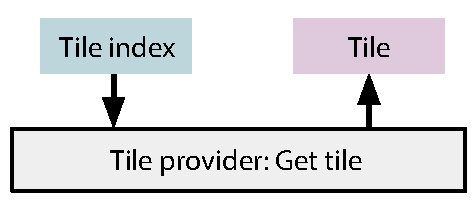
\includegraphics[width=\textwidth]{figures/implementation/tileprovider/tileprovider_gettile.pdf}
    \end{subfigure}
    \caption{Tile provider interface for accessing tiles}
    \label{fig:tileprovider}
\end{figure}

The most important functionality is the GetTile ability, which is used by client code to access the tiles. As tile providers may provide tiles of any status, the user of the tile provider is responsible to always check the status of the requested tile before using the tile. 

Several implementations of the tile provider interface were developed. They are all described below.

\subsection{Caching Tile Provider}
The \class{Caching Tile Provider} uses an \class{Async Tile Dataset} to read \class{Raw Tile}s as soon as client code tries to access a specific tile. It internally polls the \class{Async Tile Dataset} every frame for finished raw tiles. When there are ready raw tiles, the \class{Caching Tile Provider} converts the raw tiles into tiles. This is done in the initialization step which is part of the update method that is illustrated in figure \ref{fig:cachingtileprovider_update}. If no errors of the raw tile are reported, the tile gets the status ``OK'' and its texture data gets uploaded to the GPU. The tile also gets added to the in-memory cache. The functionality of accessing tiles is illustrated in figure \ref{fig:cachingtileprovider_gettile}.

The uploading of texture data to the GPU needs to be on the rendering thread since there is where the OpenGL context resides. Tiles with data uploaded to texture memory will enable it for use in rendering of a chunk.

\begin{figure}[htbp]
    \centering
    \begin{subfigure}[bt]{0.7\textwidth}
        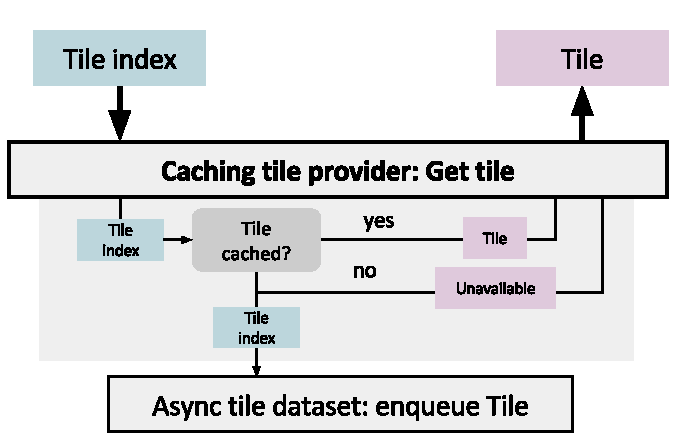
\includegraphics[width=\textwidth]{figures/implementation/tileprovider/cachingtileprovider_gettile.pdf}
    \end{subfigure}
    \caption{Tiles are either provided from cache or enqueued in an asynchronous tile dataset if it is not available}
    \label{fig:cachingtileprovider_gettile}
\end{figure}

The functionality for internally updating the tile cache is illustrated in figure \ref{fig:cachingtileprovider_update}.

\begin{figure}[htbp]
    \centering
    \begin{subfigure}[bt]{0.6\textwidth}
        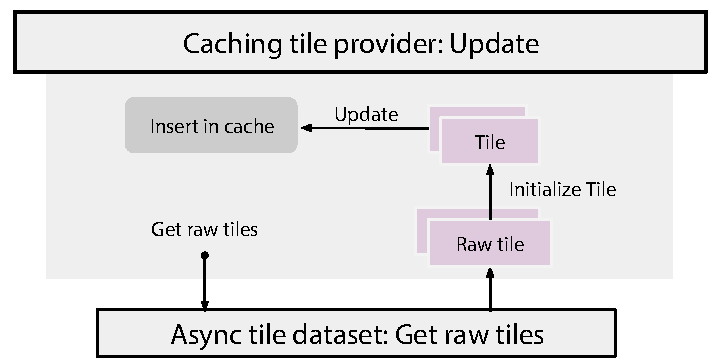
\includegraphics[width=\textwidth]{figures/implementation/tileprovider/cachingtileprovider_update.pdf}
    \end{subfigure}
    \caption{The tile cache is updated once per frame}
    \label{fig:cachingtileprovider_update}
\end{figure}

Figure \ref{fig:cachingtileprovider_tilerequest} demonstrates a typical scenario where a specific tile of index $\{3, 4, 2\}$ is requested within a sequence of render calls. The first requesting call to that tile will spawn a worker thread in the \class{Asynch Tile Dataset}. As soon as the \class{Tile} is initialized (uploaded to the GPU) and inserted in the cache, it will be accessible on the rendering thread. If the tile is not yet available the \class{Caching Tile Provider} will report that so that the calling function can continue without the use of that specific \class{Tile}.

\begin{figure}[htbp]
    \centering
    \begin{subfigure}[bt]{0.8\textwidth}
        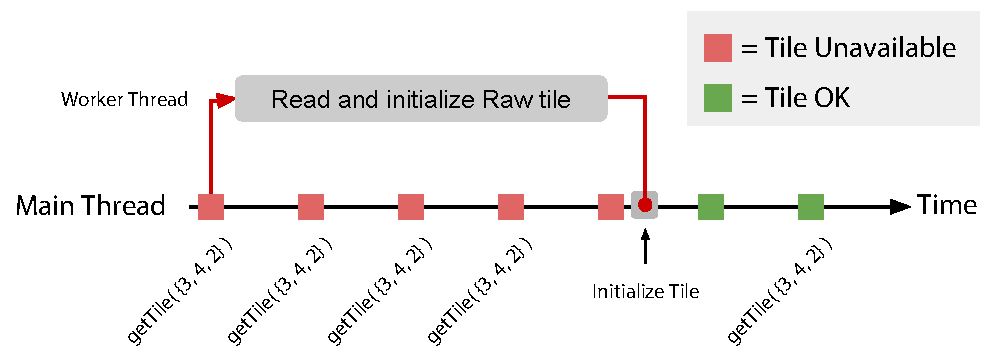
\includegraphics[width=\textwidth]{figures/implementation/tileprovider/cachingtileprovider_tilerequest.pdf}
    \end{subfigure}
    \caption{Tiles are fetched on demand. The first time a tile is requested, the asynchronous tile dataset will request it on a worker thread. As soon as the tile has been initialized it will have the status ``OK'' and can be used for rendering}
    \label{fig:cachingtileprovider_tilerequest}
\end{figure}

The caching policy implemented and used is LRU - ``Least Recently Used''. This means that tiles that have not been accessed for a while are thrown out only when the cache limit is exceeded, see section \ref{section:lrucaching} for details.

\subsection{Temporal Tile Provider}
In order to incorporate time-resolved map datasets into the rendering scheme, a tile provider for this specific purpose was implemented. The \class{Temporal Tile Provider} is instantiated with a template URI containing a time placeholder. Information about the supported time range, time resolution and expected timestamp format to be used in the template URI is also passed during instantiation. In Listing \ref{lst:temporal}, all tags starting with \texttt{OpenSpace} are used to configure information used to instantiate the temporal dataset. The tag \texttt{GDAL\_WMS} contains a functional GDAL WMS dataset specification. When requesting the URLs for the dataset, \texttt{\$\{OpenSpaceTimeId\}} will be replaced with the date and time in the specified format.

\begin{lstlisting}[language=XML,caption={Temporal WMS dataset specification} \label{lst:temporal}]
<OpenSpaceTemporalGDALDataset>
    <OpenSpaceTimeStart>2015-11-24</OpenSpaceTimeStart>
    <OpenSpaceTimeEnd></OpenSpaceTimeEnd>
    <OpenSpaceTimeResolution>1d</OpenSpaceTimeResolution>
    <OpenSpaceTimeIdFormat>YYYY-MM-DD</OpenSpaceTimeIdFormat>
    <GDAL_WMS>
        <Service name="TMS">
            <ServerUrl>
                http://datasetURL/${OpenSpaceTimeId}/${z}/${y}/${x}.jpg 
            </ServerUrl>
        </Service>
        ...
    </GDAL_WMS>
</OpenSpaceTemporalGDALDataset>
\end{lstlisting}

At runtime, the \class{Temporal Tile Provider} checks the global simulation time, quantizes that time with respect to the provided time resolution and lazily instantiates new \class{Caching Tile Provider}s per timeframe within the temporal dataset. 

A schematic illustration of the implementation of the \class{Temporal Tile Provider} is illustrated in figure \ref{fig:temporaltileprovider_gettile}.

\begin{figure}[htbp]
    \centering
    \begin{subfigure}[bt]{0.7\textwidth}
        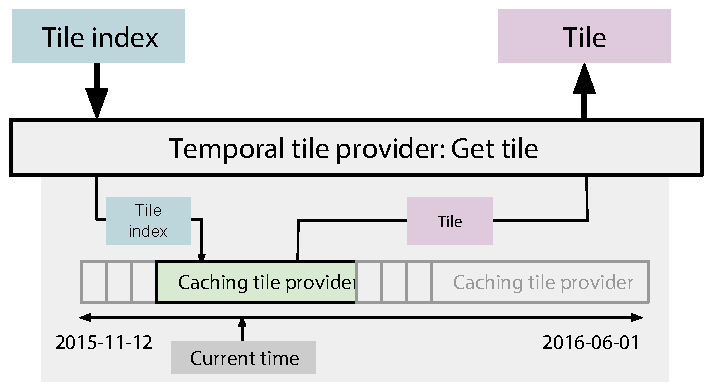
\includegraphics[width=\textwidth]{figures/implementation/tileprovider/temporaltileprovider_gettile.pdf}
    \end{subfigure}
    \caption{Each temporal snapshot is internally represented by a caching tile provider}
    \label{fig:temporaltileprovider_gettile}
\end{figure}


\subsection{Single Image Tile Provider}
This is a very simple implementation of the tile provider interface which only serves the same tile for every tile index. This tile provider was used for testing and debugging alignment and padding between tiles, see figure \ref{fig:singleimagetileprovider_gettile}.

\begin{figure}[htbp]
    \centering
    \begin{subfigure}[bt]{0.5\textwidth}
        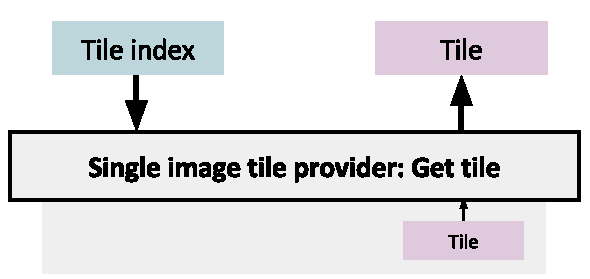
\includegraphics[width=\textwidth]{figures/implementation/tileprovider/singleimagetileprovider_gettile.pdf}
    \end{subfigure}
    \caption{Serving single tiles can be useful for debugging chunk and texture alignment}
    \label{fig:singleimagetileprovider_gettile}
\end{figure}

\subsection{Text Tile Provider}
The ability to serve tiles with text rendered on the fly was implemented as a general debugging utility. The tiles are generated on demand by rendering text to textures and cached using the same LRU caching mechanism as the \class{Caching Tile Provider}.

\begin{figure}[htbp]
    \centering
    \begin{subfigure}[bt]{0.6\textwidth}
        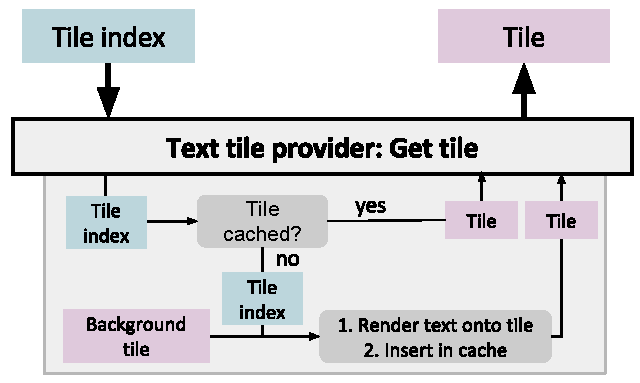
\includegraphics[width=\textwidth]{figures/implementation/tileprovider/texttileprovider_gettile.pdf}
    \end{subfigure}
    \caption{Serving tiles with custom text rendered on them can be used as size references or providing other information. The tile provider is internally holding a LRU cache for initialized tiles}
    \label{fig:texttileprovider_gettile}
\end{figure}

Two different types of \class{Text Tile Provider}s were implemented. \class{Tile Index Tile Provider} serves tiles where each tile has its tile index rendered onto it, and \class{Size Reference Tile Provider} uses the globe's reference ellipsoid to render a size reference in meters or kilometers onto its tiles.


\section{Mapping Tiles onto Chunks}
  
In the implementation of chunks suggested by Cozzi and Ring \cite{cozzi11}, chunks store the data they need for rendering by themselves. That means that as soon as a chunk has been fully initialized, it has everything it needs to be rendered. However, when dealing with multiple map datasets potentially residing on distant servers, there is no guarantee that all the tiles needed for a chunk to be rendered are available.

When an accessed \class{Tile} does not have the status ``OK'', it can not be used for rendering. The second best thing to try is to check the parent of the tile. A parent tile is guaranteed to always cover a larger geodetic map region that includes its children's subregions, but with lower number of pixels per geodetic degree. Figure \ref{fig:tiles} demonstrates this with a simple example.

\begin{figure}[htbp]
    \centering
    \begin{subfigure}[t]{0.3\textwidth}
        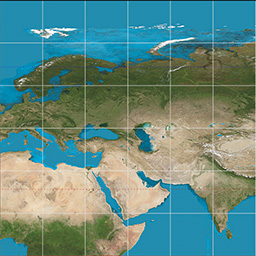
\includegraphics[width=\textwidth]{figures/implementation/chunktile/chunktile1.jpg}
        \caption{Requested tile}
    \end{subfigure}
    \quad
    \begin{subfigure}[t]{0.3\textwidth}
        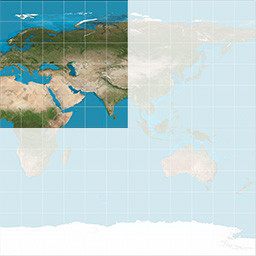
\includegraphics[width=\textwidth]{figures/implementation/chunktile/chunktile2.jpg}
        \caption{Requested tile's region shown in its parent tile}
    \end{subfigure}
    \caption{Only the highlighted subset of the parent tile is used for rendering the chunk. Figure adapted from \cite{mapprojections}}
    \label{fig:tiles}
\end{figure}

In figure \ref{fig:tiles}, it is realized that in order to use a parent tile for rendering, the texture coordinates used to sample the parent tile needs to be adjusted to represent the same geographic region. This shows the need of a higher level concept than just \class{Tile}s, which leads to the introduction of \class{Chunk Tile}s.

\subsection{Chunk Tiles}
  
A \class{Chunk Tile} represents a \class{Tile} that corresponds to a specific \class{Chunk}. It stores a \class{Tile} which is guaranteed to have the status ``OK'' along with a transform defined by a scaling and translation component. The transform is used to map texture coordinates of the chunk into its corresponding geodetic region within the tile. 

The algorithm used for selecting the highest resolution \class{Chunk Tile} from a tile provider is described by the pseudo code in Listing \ref{lst:getchunktile}.

\begin{lstlisting}[
  caption={Selecting optimal Chunk Tiles} 
  \label{lst:getchunktile}
]
ChunkTile TileSelector::getChunkTile(TileProvider* tp, TileIndex ti){
  TileUvTransform uvTransform;
  uvTransform.uvOffset = glm::vec2(0, 0);
  uvTransform.uvScale = glm::vec2(1, 1);

  while (ti.level > 1) {
      Tile tile = tp->getTile(ti);
      if (tile.status == Tile::Status::OK) {
          return { tile, uvTransform };
      }
      else {
        ascendToParent(ti, uvTransform);
      }
  }

  uvTransform.uvOffset = glm::vec2(0, 0);
  uvTransform.uvScale = glm::vec2(1, 1);
  return { Tile::TileUnavailable, uvTransform };
}
\end{lstlisting}

\iffalse
\begin{algorithm}[htp]
 \caption{Selecting optimal chunk tiles}
 \KwResult{ Chunk tile: \{Tile, UvTransform\}  }
  \SetKwProg{myalg}{GetChunkTile}{(tileProvider, tileIndex)}{}
  \myalg{}{
  \While {tileIndex.level > 0}{
      tile = tileProvider.getTile(tileIndex)
  }
  \eIf{(tile.status == OK)}{
        Return \{ tile, tileUvTransform \}
    }{
      tileUvTransform = fromParent(tileUvTransform, tileIndex);
      tileIndex.toParent();
    }
  }
  Return \{ tileProvider.defaultTile(), \{Translation: \{0,0\}, Scaling: \{1,1\} \} \}
  {}
  \label{alg:tileselection}
\end{algorithm}


\begin{algorithm}[htp]
\caption{Selecting optimal chunk tiles}
\label{alg:tileselection}
\KwResult{ A \class{ChunkTile} defined by a \class{Tile} and a \class{UvTransform}  }
  \SetKwProg{myalg}{GetChunkTile}{(\class{TileProvider}, \class{TileIndex})}{}
  \myalg{}{
    Initialize \class{UvTransform} with no scaling and no translation\\
    \While {level of \class{TileIndex} > 0}{
      Use \class{TileProvider} to access \class{Tile} at \class{TileIndex}\\
      \eIf{(\class{Tile} has status OK)}{
        \Return \class{ChunkTile} defined by \class{Tile} and \class{UvTransform}\\
      }{
        Modify \class{UvTransform} and \class{TileIndex} to represent the same geographic region at a higher mip level
      }
    }
    Use \class{TileProvider} to access the \class{Default Tile}\\
    Let \class{UvTransform} have no scaling and no translation\\
    \Return \class{ChunkTile} defined by \class{Default Tile} and \class{UvTransform}\\
  }
  {}
\end{algorithm}
\fi

 
The subroutine \texttt{ascendToParent} returns an updated transform which maps texture coordinates to the same geodetic region within the next parent tile. The routine is described in Listing \ref{lst:ascendtoparent}.

\begin{lstlisting}[caption={Ascend to parent} \label{lst:ascendtoparent}]
void TileSelector::ascendToParent(TileIndex& tileIndex, TileUvTransform& uv) {
    uv.uvOffset *= 0.5;
    uv.uvScale *= 0.5;

    if (tileIndex.isEastChild()) {
        uv.uvOffset.x += 0.5;
    }

    // In OpenGL, positive y direction is up
    if (tileIndex.isNorthChild()) {
        uv.uvOffset.y += 0.5;
    }

    tileIndex.toParent();
}
\end{lstlisting}

\iffalse
\begin{algorithm}[htp]
 \caption{Get the transform from the parents texture coordinates}
 \KwResult{ UvTransform: \{Translation, Scaling\}  }
  \SetKwProg{myalg}{fromParent}{(tileUvTransform, tileIndex)}{}
  \myalg{}{
      tileUvTransform.translation *= 0.5
      tileUvTransform.scaling *= 0.5
  \If{(tileIndex is an eastern child)}{
        tileUvTransform.translation.x += 0.5
    }
    \If{(TileIndex is a northern child)}{
        tileUvTransform.translation.y += 0.5
    }
  }
  Return tileUvTransform
  {}
  \label{alg:fromparent}
\end{algorithm}

The subroutine \texttt{getParent} simply returns the parent of the provided tile index as described in Algorithm \ref{alg:parent}.

\begin{algorithm}[htp]
 \caption{Get the parent tile index}
 \KwResult{ TileIndex: \{level, x, y\}  }
  \SetKwProg{myalg}{TileIndex::Parent}{}{}
  \myalg{}{
  Return \{level-1, x/2, y/2\}
  }{}
  \label{alg:parent}
\end{algorithm}
\fi

As opposed to regular tiles, chunk tiles can always be used for rendering since they by definition always have the status ``OK''.

\subsection{Chunk Tile Pile}
\label{section:chunktilepile}

A \class{Chunk Tile Pile} represents a range of \class{Chunk Tile}s across multiple mip levels. They contain the information needed to perform the LOD switching later described under section \ref{section:lodswitching}. Retrieving a \class{Chunk Tile Pile} simply requires a tile index of the highest desired mip level (highest LOD) and the number of desired \class{Chunk Tile}s in the pile as described in Listing \ref{lst:chunktilepile}.

\iffalse
\begin{algorithm}[htp]
 \caption{Get a chunk tile for a specific tile index}
 \KwResult{ ChunkTilePile }
  \SetKwProg{myalg}{getChunkTilePile}{(tileProvider, tileIndex, pileSize)}{}
  \myalg{}{
  chunkTilePile = [ ] \\
  \For{i in range [1, pileSize]}{
  	chunkTilePile.append(getChunkTile(tileIndex)) \\
  	tileIndex = tileIndex.parent()
  }
  Return chunkTilePile
  }{}
  \label{alg:getchunktilepile}
\end{algorithm}
\fi

\begin{lstlisting}[caption={Instantiating a Chunk Tile Pile} \label{lst:chunktilepile}]
ChunkTilePile TileSelector::getChunkTilePile(TileProvider* tp, TileIndex ti, int n){
  ChunkTilePile chunkTilePile;
  for (int i = 0; i < n; ++i){
    chunkTilePile.push_back(getChunkTile(tp, ti));
    ti.toParent();
  }
  return chunkTilePile;
}
\end{lstlisting}

As an example: 
Assuming that the texture data is available in local memory, invoking the getChunkTilePile method with index $\{x: 2240, y: 4824, level: 13 \}$ and a chunk tile pile size 3, would return the \class{Chunk Tile Pile} represented in figure \ref{fig:chunktilepile}. 

\begin{figure}[htbp]
    \centering
    \begin{subfigure}[t]{0.3\textwidth}
        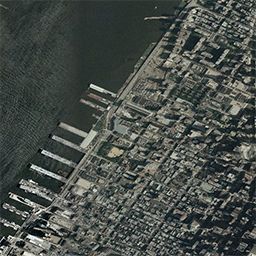
\includegraphics[width=\textwidth]{figures/implementation/chunktile/chunktilepile3.png}
        \caption{Tile}
    \end{subfigure}
    \quad
    \begin{subfigure}[t]{0.3\textwidth}
        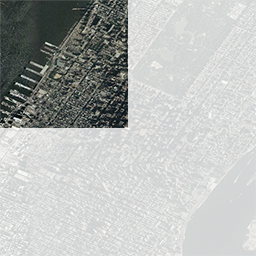
\includegraphics[width=\textwidth]{figures/implementation/chunktile/chunktilepile2.png}
        \caption{Parent 1}
    \end{subfigure}
    \quad
    \begin{subfigure}[t]{0.3\textwidth}
        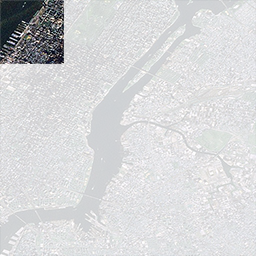
\includegraphics[width=\textwidth]{figures/implementation/chunktile/chunktilepile1.png}
        \caption{Parent 2}
    \end{subfigure}
    \caption{The image data of a given chunk tile pile. Only the highlighted subset of the parent tiles are used for rendering the chunk. Figure from \cite{imageryworld2d}}
    \label{fig:chunktilepile}
\end{figure}

As chunk tiles are guaranteed to be good for rendering on the GPU (since their tiles are guaranteed to have the status ``OK''), all \class{Chunk Tile Pile}s are guaranteed to be good for rendering as well. 

\section{Managing Multiple Data Sources}
The \class{Layer Manager} maintains and organizes different types of texture data sources into groups. This is required as different types of texture datasets are used for different purposes and thus rendered in different ways. The \class{Layer Manager} owns seven \class{Layer Groups}; these are:

\begin{enumerate}
\item Heightmaps
\item ColorLayers
\item ColorOverlays
\item GrayScaleLayers
\item GrayScaleOverlays
\item NightLayers
\item WaterMasks
\end{enumerate}

\subsection{Layers}
Much like in image editing softwares, a layer in this context represents a raster of pixels, which among other internally ordered raster of pixels, are used to produce a final result. A \class{Layer} consists of three things:

\begin{enumerate}
\item A \class{Tile Provider} - Used for accessing tiles of texture data.
\item A collection of render settings for real time image processing. The parameters implemented at this stage are \emph{gamma}, \emph{multiplier} and \emph{opacity}.
\item A simple boolean property which specifies whether the layer is enabled or disabled. Disabled layers are not used in rendering.
\end{enumerate}

\class{Layer}s allow for retrieving of \class{Chunk Tile Pile}s, as described in section \ref{section:chunktilepile}. The class hierarchy and data flow is illustrated in figure \ref{fig:layermanager}.

\begin{figure}[htbp]
    \centering
    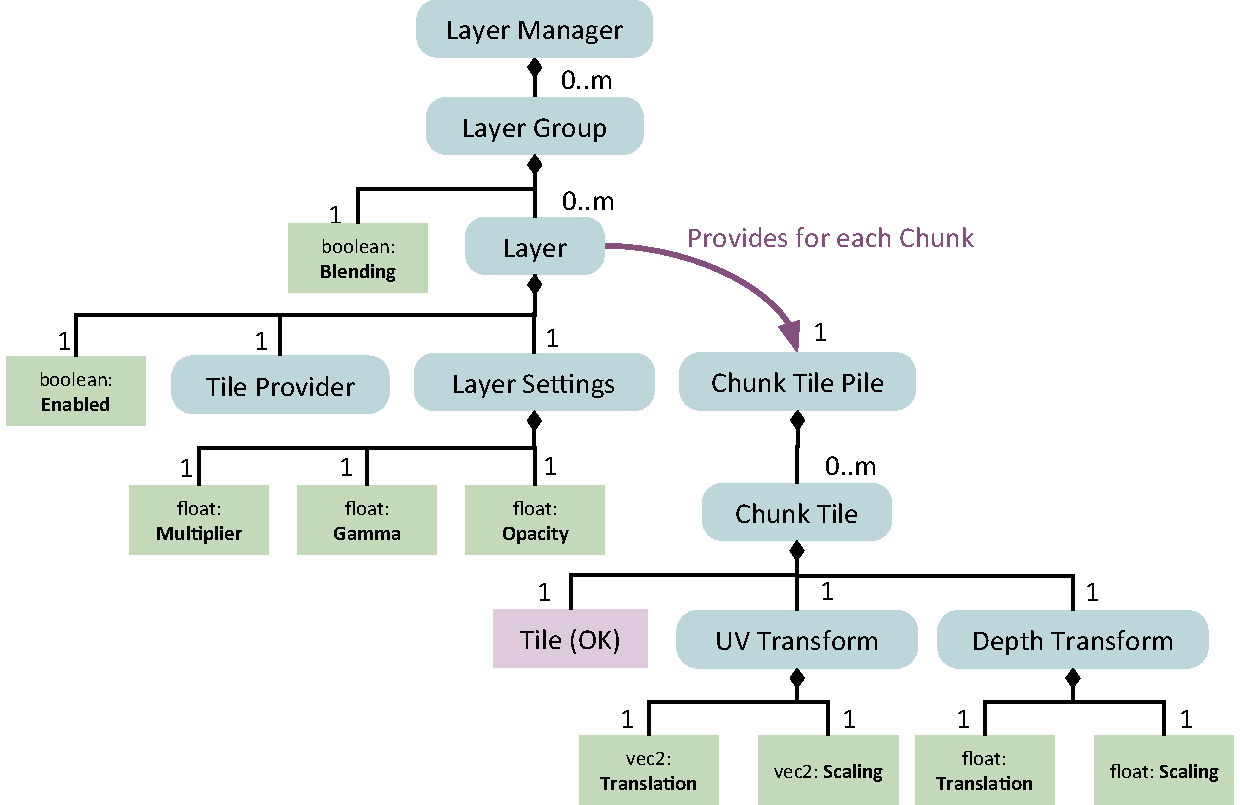
\includegraphics[width=\textwidth]{figures/implementation/layers/layermanager.pdf}
    \caption{UML diagram of the \class{Layer Manager} and its related classes}
    \label{fig:layermanager}
\end{figure}

\subsection{Layers on the GPU}

The data hierarchy defined by \class{Layer Manager} can almost be reproduced on the GPU by using GLSL in a near object-oriented approach. In order to handle the data mapping between the CPU and GPU, a CPU representation for the GPU data was implemented. This allows for updating the values of uniform variables and map uniform names to uniform locations.

\subsubsection{CPU to GPU Data Mapping}

There are some key differences between the \class{Layer Manager} data structure on the CPU and its corresponding GPU-synchronized representation - \class{GPU Layer Manager}. These are:

\begin{itemize}
\item The GPU representation does not store any of the actual \class{Layer} data - only the uniform locations within a shader program so that it knows where to upload the layer data to the GPU. 
\item Render calls are done on a per chunk basis. This means that all texture data to be used within a single render call is contained in a single \class{Chunk Tile Pile} for each \class{Layer}. Thus, the \emph{provides}-relation between \class{Layer} and \class{Chunk Tile Pile} in figure \ref{fig:layermanager} simply becomes a \emph{has}-relation between a \class{GPU Layer} and a \class{GPU Chunk Tile Pile}.
\item Layers that are disabled are not rendered, and consequently not uploaded to the GPU. This means that all layers on the GPU are enabled, thus they do not need to store that information.
\end{itemize}

Incorporating these few differences yields a similar class hierarchy, as illustrated in figure \ref{fig:gpulayermanager}. 

\begin{figure}[htbp]
    \centering
    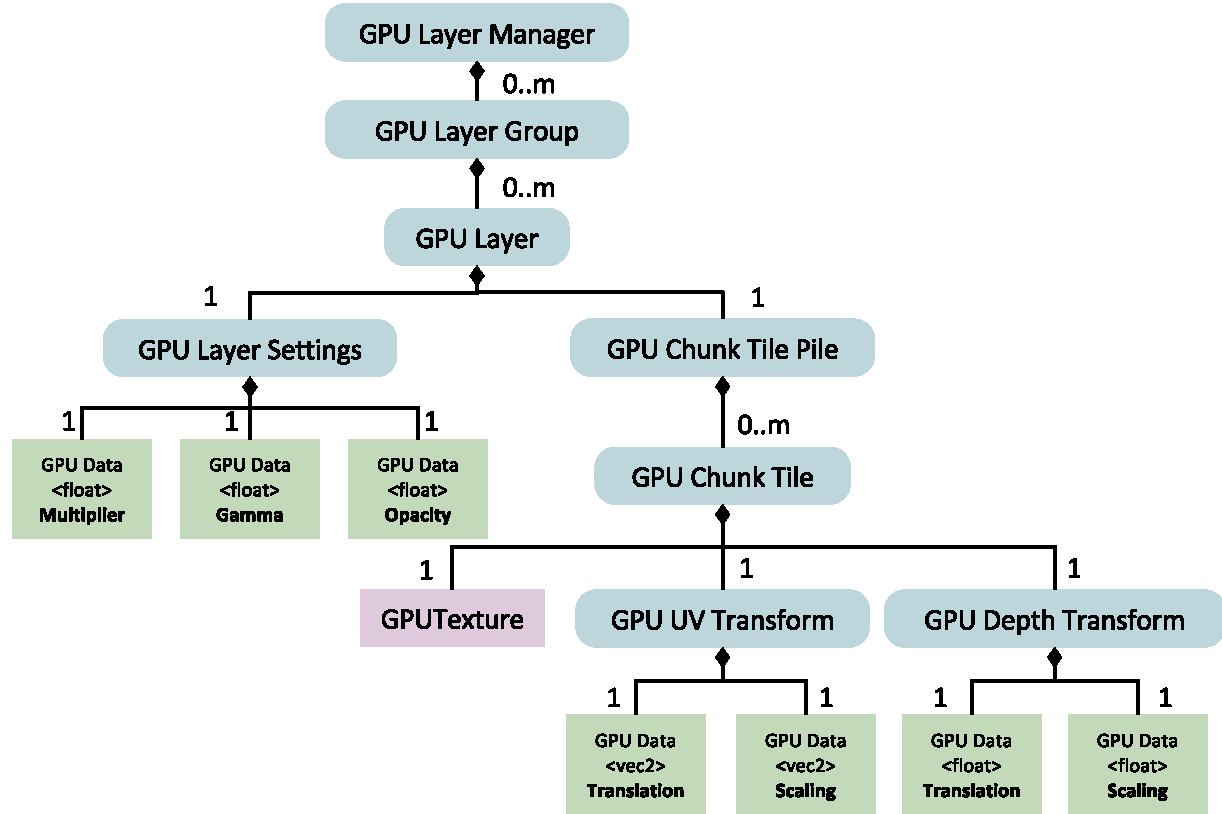
\includegraphics[width=\textwidth]{figures/implementation/layers/gpulayermanager.pdf}
    \caption{UML structure for corresponding GPU-mapped hierarchy. The class \texttt{GPUData<T>} maintains an OpenGL uniform location}
    \label{fig:gpulayermanager}
\end{figure}

The leaf classes within the class hierarchy store one uniform location each and represent one GLSL uniform value. The declaration of the layer uniforms within the shader code is defined so that it matches the exact same hierarchy. This is implemented by mapping C++ classes to GLSL structs and representing \emph{one-to-many} relationships as structs with a range of conformly named fields, or plain GLSL arrays.

\subsubsection{Updating the GPU Data}

With this 1:1 data mapping between the CPU and GPU, all the GPU-prefixed classes were given two responsibilities.

\begin{enumerate}
\item Bind its uniform locations to GLSL variable names within a provided shader program
\item Set its uniform values within a provided shader program. That is, a \class{GPU Chunk Tile} should be able to set its uniform values from a regular \class{ChunkTile}
\end{enumerate}

The leaf classes automatically takes care of both binding its uniform location to specific GLSL variables and  setting their uniform values. The compound GPU-prefixed classes (non leaf classes) more or less simply propagates the method calls to all its dependents. When binding an object to a variable name, the GLSL variable identifiers are built up successively during the propagation down to the leaf classes. \class{GPU Layer} is used as an example in Listing \ref{lst:bindgpulayer}.

\begin{lstlisting}[
  caption={Bind a GPU Layer to a Layer on the CPU} 
  \label{lst:bindgpulayer}
]
void GPULayer::bind(ProgramObject* p, std::string nameBase, int pileSize){
	this->gpuChunkTilePile.bind(p, nameBase + "pile.", pileSize)
	this->gpuRenderSettings.bind(p, nameBase + "settings.")
}
\end{lstlisting}

In Listing \ref{lst:bindgpulayer}, it can be concluded that each layer in the GLSL code must be a struct with a member called ``pile'' and a member called ``settings''. An example of a fully resolved identifier is: 

\begin{lstlisting}[]
"ColorLayers[0].pile.chunkTile0.tileUvTransform.scaling"
\end{lstlisting}

When setting the values, the GPU representation of the data is updated based on the currently available \class{Layer} data, and the update is propagated down to all the leaf classes. This is exemplified using code from the \class{GPULayer} class defined in Listing \ref{lst:gpulayersetvalue}.

\begin{lstlisting}[
  caption={Set all GPU Layer variables from a CPU Layer} 
  \label{lst:gpulayersetvalue}
]
GPULayer::setValue(ProgramObject* p, Layer& l, TileIndex ti, int n){
	ChunkTilePile chunkTilePile = l.getChunkTilePile(ti, n);
	this->gpuChunkTilePile.setValue(p, chunkTilePile);
	this->gpuRenderSettings.setValue(p, l.renderSettings());
}
\end{lstlisting}

\section{Chunk Rendering}

Given the ability to specify and use different layers to be used for rendering and the actual chunks that need to be visible, they are ready to be rendered. Rendering includes using vertex- and fragment shaders when invoking a rendering call on a given geometry; in this case, a grid.

\subsection{Grid}

A chunk grid is defined by a number of segments $N$ in two dimensions, which is used to build up a two dimensional array of vertex coordinates. These vertex coordinates can be used both for texture fetching and as interpolation parameters in an inverse geographic projection function to place a each vertex in 3D space. Figure \ref{fig:grid} shows how a surrounding region have coordinate values less than 0 or greater than 1 in either the $u$ or the $v$ dimension. This region is referred to as the skirt of the grid and it is offset in the vertical direction in the vertex shaders to cover cracks between chunks.

\begin{figure}[htbp]
    \centering
    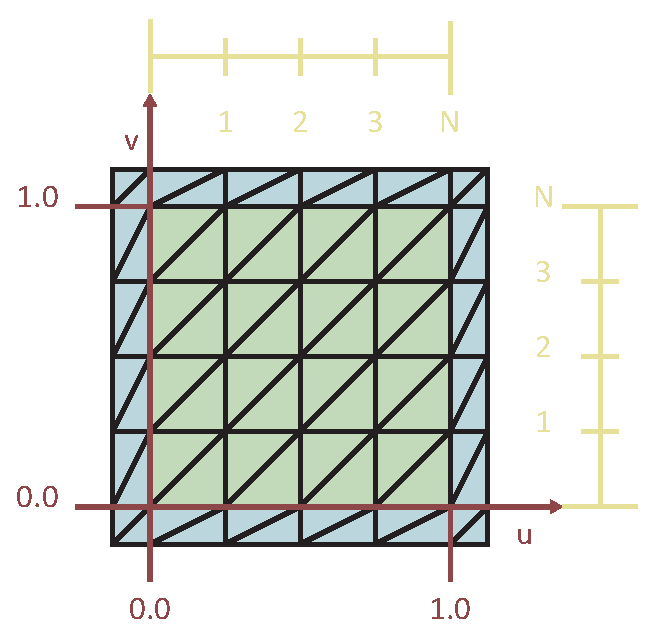
\includegraphics[width=0.5\textwidth]{figures/implementation/rendering/grid.pdf}
    \caption{Grid with skirts with a side of $N=4$ segments. Green represents the main area with texture coordinates $\in \left[  0, 1 \right] $ and blue is the skirt of the grid}
    \label{fig:grid}
\end{figure}

\subsection{Vertex Pipeline}

The grid can be rendered using different methods to weight precision against accuracy. In the vertex shader, the vertex positions are set so that the chunk geometry can be rasterized and rendered as a mesh on the screen. Height mapping is performed by offsetting vertices in the direction of the geodetic normals on the GPU which means that vertex texture fetching is needed in the rendering pipeline.

The mapping from geodetic coordinates to cartesian model space coordinates can be done on the GPU in single precision to position vertices on the globe. As discussed in section \ref{section:precision}, however, this is not sufficient to achieve sub meter precision on an Earth sized globe.

\subsubsection{High Precision Rendering}

The first step in avoiding precision errors is what Cozzi and Ring refers to as rendering relative to center \cite{cozzi11}. In short, it boils down to calculating the model-view matrix in double precision on the CPU side and then casting the matrix to a single precision representation before uploading it to the GPU. This method works well for small objects where the vertices positioned close to the origin (center) of the model \cite{cozzi11}. For planet sized objects, we need to go further than that.

One method that works for all models but can be considered naive as the number of vertices increases is what Cozzi and Ring refers to as CPU relative to eye rendering. By using a dynamic vertex buffer, all vertex positions can be transformed to camera space in double precision before being cast to single precision and dynamically uploaded to the GPU. This method becomes very tedious if the number of vertices is big. However, since the mesh of a chunk is essentially an ellipsoid segment, the whole mesh can be interpolated using a limited number of control points.

We have considered two different categories of rendering techniques: model space rendering and camera space rendering. The techniques can be implemented differently and used at different scales to accommodate for flexibility, accuracy and precision.

\subsubsection{Model Space Rendering}

The most straightforward method for rendering geodetic chunks is to transform the geodetic coordinates of each vertex to cartesian model space coordinates using the inverse geographic projection transform, $P^{-1}(\phi, \theta)$, in the vertex shader. An affine transform can be applied to the vertex coordinates by knowing the geodetic coverage of the chunk. It can be derived from the chunk's tile index. The inverse projection transform is performed with limited precision floating point operations on the GPU but the accuracy will be high as vertices will be positioned exactly on the globe in geodetic coordinates. Figure \ref{fig:global}.

\begin{figure}[htbp]
    \centering
    \begin{subfigure}[tb]{0.3\textwidth}
    	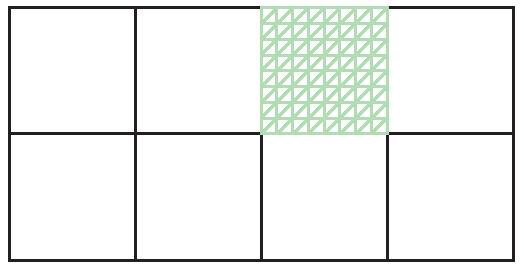
\includegraphics[width=\textwidth]{figures/implementation/rendering/gridmap.pdf}
    \end{subfigure}
    \begin{subfigure}[tb]{0.4\textwidth}
    \begin{picture}(50,50)
        \put(25,25){$\left( \begin{matrix} x \\ y \\ z \end{matrix} \right) =P^{ -1 }(\phi ,\theta )\rightarrow$}    
    \end{picture}
    \end{subfigure}
    \begin{subfigure}[tb]{0.2\textwidth}
    	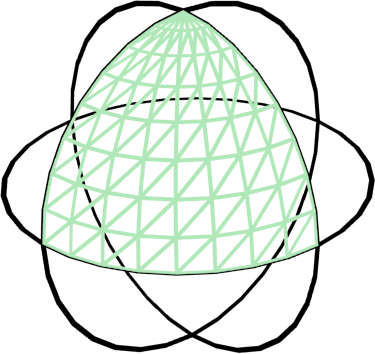
\includegraphics[width=\textwidth]{figures/implementation/rendering/gridonglobe.png}
    \end{subfigure}
    \caption{Model space rendering of chunks is performed with a mapping of vertices from geodetic coordinates to cartesian coordinates.}
    \label{fig:global}
\end{figure}

The model space rendering method essentially achieves the same precision as rendering a predefined chunk mesh relative to the center of mass of the globe. Figure \ref{fig:pipelineglobal} shows the pipeline for rendering a chunk using the model space method.

\begin{figure}[htbp]
    \centering
    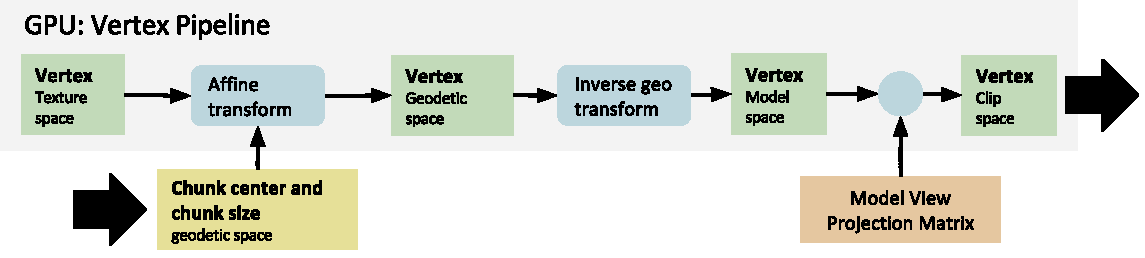
\includegraphics[width=\textwidth]{figures/implementation/rendering/pipeline_global.pdf}
    \caption{Vertex pipeline for model space rendering. Variables on the CPU are defined in double precision and cast to single precision before being uploaded to the GPU}
    \label{fig:pipelineglobal}
\end{figure}

\subsubsection{Camera Space Rendering}

Camera space rendering is performed by transforming only a limited number of control points for each chunk to camera space using double precision arithmetics. Once in camera space, the points can be cast to single precision and used for interpolation on the GPU to get all the final vertex positions of the chunk. Having the points in camera space solves the proposed precision issues since the precision will increase when the points are closer to the camera. This concept is illustrated in figure \ref{fig:local} where the vertex position vector precision increases as vertices are closer to the camera.

\begin{figure}[htbp]
    \centering
    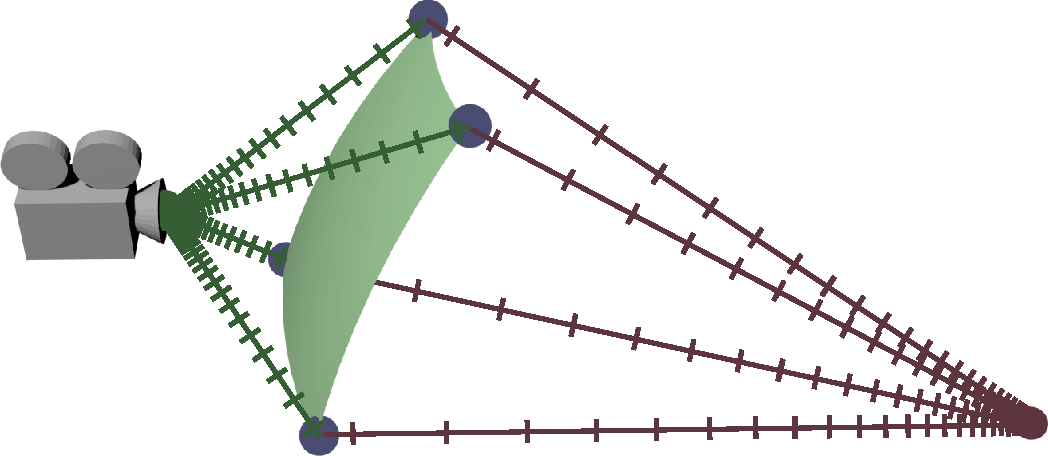
\includegraphics[width=0.5\textwidth]{figures/implementation/rendering/local.pdf}
    \caption{Interpolating vertex positions in camera space leads to high precision in the representation of vertex positions close to the camera compared to positions defined in model space.}
    \label{fig:local}
\end{figure}

\paragraph{Chunks as NURBS Surfaces}
Non Uniform Rational B-Splines (NURBS) can represent all conic sections exactly which is important for modelling ellipses in the 1D case and ellipsoids in the 2D case. A geodetic chunk can be uniquely defined by nine control points which can be calculated using the tile index representing the chunk.

The positive aspect about rendering geodetic chunks as NURBS surfaces is that it is a unified way of rendering chunks and that the precision works for all scales. Chunks will always be mapped exactly on the ellipsoid and the precision will increase when the camera gets closer. However, the negative aspect that makes NURBS insufficient for texture mapped globes is the fact that the texture coordinates of the vertices do not linearly map to the geodetic coordinates of the chunk. In other words, vertices are not evenly distributed along the surface of the chunk which leads to distorted textures. The reason for this is the fact that NURBS are rational parametric functions. For example, a circle segment can be represented exactly but a given parameter value will not yield the same position along a circle segment as a circle segment parameterized as $\{x(t),y(t)\} = \{cos(t), sin(t)\}$. The $cos$ and $sin$ functions are irrational and can therefore not be represented with NURBS segments which by definition are rational.

\paragraph{Chunks as Bilinear Surfaces}
To avoid both the texture distortion of NURBS and the precision issues of model space rendering, we use a different method for rendering chunks that are closer to the camera and hence require higher precision. When the camera gets closer to the surface of the ellipsoid, the chunks will split and get smaller according to the chunk selection under Section \ref{section:chunkselection}. Smaller patches will automatically be better approximated as flat surfaces so that at a certain level, before the precision errors of the global patches become predominant, the rendering of patches can be switched to the a camera space rendering method which uses bilinear interpolation of vertex positions.

This method is performed by, just as in the case of NURBS surfaces, transforming control points from cartesian model space to camera space where they can be cast to single precision representations. Instead of NURBS interpolation, a simple bilinear interpolation is used to place all the vertices on the surface defined by the four corner points of the patch that covers the chunk.

With bilinear interpolation, high precision is achieved for vertices placed close to the camera. Also, the vertices will be uniformly spaced which means that the textures will not be distorted. Worth noticing is that if bilinear interpolation rendering is performed on chunks with low level, the approximation will be less accurate. Switching to camera space rendering with bilinear interpolation at level 10 gives a reasonable balance between the ellipsoidal mapping of the model space rendering and the high precision of the camera space chunk rendering.

\todo[inline]{Maybe have a discussion in the Discussion chapter about measuring the error of using bilinear surfaces at different levels.}

Figure \ref{fig:pipelinelocal} shows a flowchart of the local vertex rendering pipeline.

\begin{figure}[htbp]
    \centering
    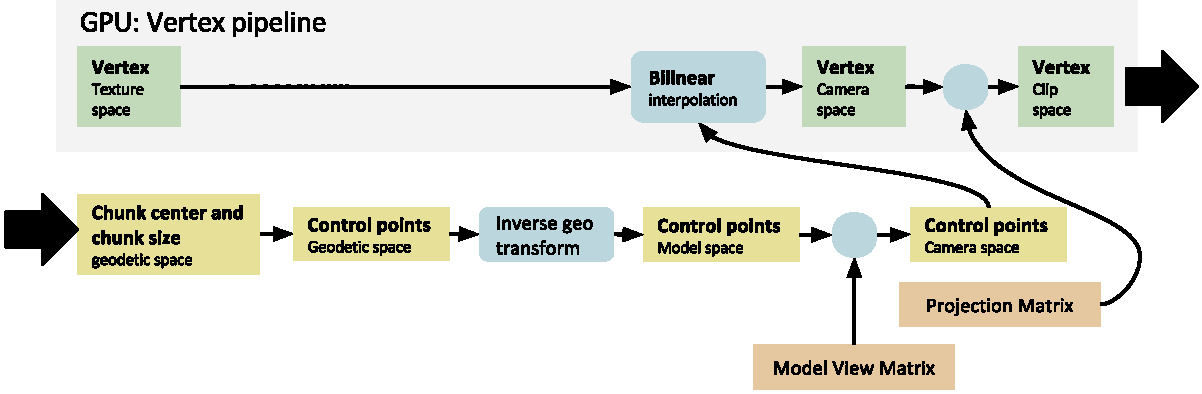
\includegraphics[width=\textwidth]{figures/implementation/rendering/pipeline_local.pdf}
    \caption{Vertex pipeline for camera space rendering. Variables on the CPU are defined in double precision and cast to single precision before being uploaded to the GPU}
    \label{fig:pipelinelocal}
\end{figure}

\subsection{Fragment Pipeline}

The purpose of layered texture rendering is to provide the user an ability to toggle different kinds of layers for rendering a chunk. For each fragment, the final color is calculated by using the active layer groups. This is done using the following step in the fragment shader which is the same for the camera space rendered chunks as it is for the model space rendered chunks:


\begin{enumerate}
\item \textbf{For all ColorLayers}: Sample RGB, apply layer settings and update fragment RGBA using alpha blending
\item \textbf{For all GrayscaleLayers}: Sample the grayscale value R, apply layer settings and update fragment V in color space HSV using alpha blending
\item \textbf{For all GrayscaleOverlays}: Sample grayscale value R and A, apply layer settings and update fragment RGBA using alpha blending
\item \textbf{For all WaterMasks}: Sample A, apply layer settings and add A as a specularity component for the fragment
\item \textbf{For all NightTextures}: Sample RGB, apply layer settings and update fragment RGBA using alpha blending in shaded regions of the globe
\item Perform shading by darkening shaded regions
\item Add simple atmosphere color to RGB
\item \textbf{For all ColorOverlays}: Sample RGBA, apply layer settings and update fragment RGBA using alpha blending

\end{enumerate}

All of these steps are optional and can be toggled by activating or deactivating layers or specifying whether or not to perform shading or use atmosphere for rendering. Sampling the color from a layer group is done by looping through all layers in that group, see Listing \ref{lst:loopthroughlayers}. Listing \ref{lst:gettexval1} and \ref{lst:gettexval2} shows how layer weights and texture transforms for chunk tile piles are used for sampling of the tile textures. Layer settings is performed for all raster bands within all layers. The application of layer settings is shown in Listing \ref{lst:performsettings}.

\begin{lstlisting}[
  caption={Setting color for a given layer group. Example using ColorLayers} 
  \label{lst:loopthroughlayers}
]
#for i in 0..#{lastLayerIndexColorLayers} {
		vec4 colorSample = getTexVal(ColorLayers[#{i}].pile,
			levelWeights, uv);
		colorSample = performLayerSettings(colorSample,
			ColorLayers[#{i}].settings);
		color = blendOver(color, colorSample); // Alpha blending
	}
#endfor
\end{lstlisting}

\begin{lstlisting}[
  caption={Getting texture value by blending a chunk tile pile} 
  \label{lst:gettexval1}
]
vec4 getTexVal(ChunkTilePile chunkTilePile, LevelWeights w, vec2 uv){
	return w.w1 * getTexVal(chunkTilePile.chunkTile0, uv) + 
		w.w2 * getTexVal(chunkTilePile.chunkTile1, uv) + 
		w.w3 * getTexVal(chunkTilePile.chunkTile2, uv);
}
\end{lstlisting}

\begin{lstlisting}[
  caption={Using texture transform and sampling a texture} 
  \label{lst:gettexval2}
]
vec4 getTexVal(ChunkTile chunkTile, vec2 tileUV){
	vec2 samplePosition = TileUVToTextureSamplePosition(chunkTile, tileUV);
	vec4 texVal = texture(chunkTile.textureSampler, samplePosition);
	return texVal;
}
\end{lstlisting}


\begin{lstlisting}[
  caption={Perform layer settings} 
  \label{lst:performsettings}
]
float performLayerSettings(float currentValue, const LayerSettings settings) {
	float newValue = currentValue;
	newValue = sign(newValue) * pow(abs(newValue), settings.gamma);
	newValue = newValue * settings.multiplier;
	newValue = newValue * settings.opacity;
	return newValue;
}
\end{lstlisting}

\subsection{Dynamic Shader Programs}

The ability to dynamically toggle layers with dynamic blending requires multiple sampling of textures in the fragment shaders. To avoid unnecessary processing when not all layers are in use there is a need to dynamically recompile the shader programs as layers are toggled. We use the GLSL preprocessor in the General Helpful Open Utility Library (GHOUL) \cite{ghoul} to preprocess all shader programs when the number of layers in use change.

We define a layer shader program to be a GLSL program object using vertex and fragment shading. Moreover, it fits the pipeline of rendering a chunk with a specific number of layer groups and a varying number of layers for each group.

To decide whether or not a layer shader program needs to be preprocessed and re-compiled, the relevant Layer Shader Preprocessing Data is saved for the layer shader program and compared to the updated preprocessing data if it has been changed by the user. Table \ref{table:layergrouppreprocessingdata} shows what data is needed to preprocess layer shader programs. Key-value pairs can be used to set properties that are used on a per-globe basis. Examples are \textbf{performShading} : \emph{true} or \emph{false}, \textbf{useAtmosphere} : \emph{true} or \emph{false}. Letting the preprocessor handle these properties avoids the need of uniform variable uploading and GLSL if-statements. The preprocessor also handles unrolling of for-loops which go through all layers in a group, see Listing \ref{lst:loopthroughlayers}.


\begin{table}
\centering 
\caption[]{Data used for a layer group for preprocessing of layer shader programs}
\label{table:layergrouppreprocessingdata}
\begin{tabular}{ c }    
    	\hline
        \textbf{Layer Group Preprocessing Data} \\ 
    	\hline
	Number of layers: integer \\
    	Blending enabled: boolean \\
	\hline
\end{tabular}
\end{table}

\begin{table}
\centering
\caption[]{Data used for a renderable globe for preprocessing of layer shader programs}
\label{table:layergrouppreprocessingdata}
\begin{tabular}{ c }
    
    	\hline
        \textbf{Layer Shader Preprocessing Data} \\ 
    	\hline
	0..* Preprocessing data: Layer Group Preprocessing Data \\
    	0..* Key-value pairs: pair of strings \\
    	\hline
    
\end{tabular}
\end{table}

\subsection{LOD Switching}
\label{section:lodswitching}
Instead of the time based switching routine proposed by Cozzi and Ring \cite{cozzi11}, we perform a distance based switching which works on a per fragment basis for textures and on a per vertex basis for height maps. The method is implemented in the vertex and fragment shaders and uses linear interpolation between levels. The blending technique uses the concept of Chunk Tile Piles as seen in section \ref{section:chunktilepile}. A Chunk Tile Pile contains three chunk tiles of different level to achieve level blending which is used to avoid popping artifacts. 

When rendering a specific fragment of a chunk, blending between up to three chunk levels can be used as a part of the switching in the chunked LOD algorithm. Assuming that the level of Tile 0 is equal to the level of the chunk to render and that Chunk Tile 1 and Chunk Tile 2 are 1 and 2 levels lower respectively, three level weights can be determined based on the distance to the fragment to achieve smooth transitions between levels. The three level weights are based on an interpolation parameter $t$ as in Listing \ref{lst:levelweights}.

\begin{lstlisting}[
  caption={Calculate level weights for three chunk tiles using an interpolation parameter calculated based on the distance between the camera and the fragment}
  \label{lst:levelweights}
]
LevelWeights getLevelWeights(float t){ // level interpolation parameter
	LevelWeights levelWeights;
	levelWeights.w1 = clamp(1 - t, 0 , 1);
	levelWeights.w2 = clamp(t, 0 , 1) - clamp(t - 1, 0 , 1);
	levelWeights.w3 = clamp(t - 1, 0 , 1);
	return levelWeights;
}
\end{lstlisting}

The interpolation parameter $t$ is calculated using the distance to the camera $d$ and the current level of the chunk $l$ as in equation \ref{eq:interpolation}.

\begin{equation}
\label{eq:interpolation}
t = l-log_2(\frac{s}{d}),
\end{equation}

where $s$ is a scale factor determining how much of the higher level tile to use in the blending. In the ideal case, the interpolation parameter should be a value between 0 and 1. However, adjacent chunks can have a difference in level greater than 1 which in turn leads to interpolation parameters with larger values. This is why it is not enough with two Chunk Tiles per Chunk Tile Pile to guarantee no popping. Popping can also occur if the LOD scale factor $s$ is small enough for adjacent chunks to have even bigger difference in level. Figure \ref{fig:switchingblending} shows how the interpolation parameter from the desired level is used for blending between tiles of different level.

\begin{figure}[htbp]
    \centering
    \begin{subfigure}[tb]{0.49\textwidth}
    	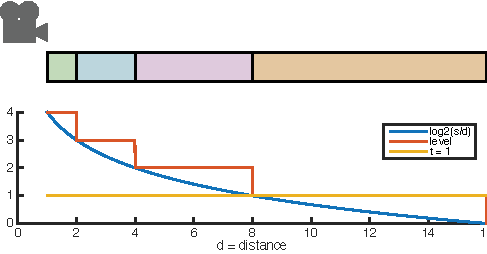
\includegraphics[width=\textwidth]{figures/implementation/rendering/blending1.pdf}
	\caption{Blending disabled}
    \end{subfigure}
    \begin{subfigure}[tb]{0.49\textwidth}
    	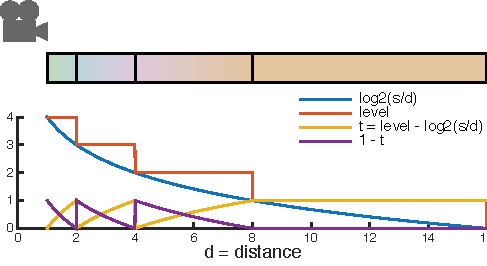
\includegraphics[width=\textwidth]{figures/implementation/rendering/blending2.pdf}
	\caption{Blending enabled}
    \end{subfigure}
    \caption{Blending on a per fragment basis. The level interpolation parameter $t$ is used to calculate level weights $w_1 = 1-t$ and $w_2 = t$, in this case using two chunk tiles per chunk tile pile.}
    \label{fig:switchingblending}
\end{figure}

\section{Interaction}

An interaction mode specifically for globe browsing had to be implemented to deal with the vast scale differences and limitations of camera movements required for browsing globes. 

Representing the camera state as a three dimensional cartesian vector for the position and a quaternion for the rotation made it possible to achieve interaction solving the proposed objectives. Basic linear algebra was used on vectors such as the geodetic normal of the globe in the camera position geodetically projected on the surface, camera position and direction as well as the height offset of the terrain.

The horizontal movement interaction speed was set to be proportional to the distance from the camera to the terrain surface. That way the user can come in close and slowly hover across the detailed terrains as well as quickly moving from one continent to the other by increasing the height to the surface.

The camera rotation quaternion can be decomposed in to two rotations; one directing the camera in the direction of the geodetic normal, and one directing it in the remaining view direction with a given roll. This way it is possible to both travel across the surface and keeping the horizon angle as well as looking around at the spot.

The camera is always pushed up above the surface of the terrain to avoid penetrating it. The minimum height given in meters can be set together with other parameters such as sensitivity and friction.
